\section{\textsc{IntraCFG}: Intraprocedural Framework for Source-Level Control-Flow Analysis}
The techniques of CFGs construction has seen significant advancements
in recent years, with various frameworks being proposed to aid in the construction 
of precise intraprocedural CFGs~\cite{smits2020flowspec,10.1016/j.scico.2012.02.002}.
We contributed to the state-of-the-art introducing \textsc{IntraCFG}, a declarative, RAG-based,
and language-independent framework for constructing precise intraprocedural CFGs.

Unlike most other frameworks, which build CFGs on an Intermediate Representation (IR) level,
such as bytecode, \textsc{IntraCFG}'s approach is unique in that it superimposes the CFGs 
on the Abstract Syntax Tree (AST). This allows for a more accurate client analysis,
as the CFGs are constructed directly on the source code level, rather than an
intermediate representation. Additionally, this approach also enables the construction 
of \textsc{AST-Unrestricted} CFGs, which are CFGs whose shape is not restricted to the AST structure.
\subsection{Overall Architecture}
The overall architecture of our proposed framework, \textsc{IntraCFG}, and its
ecosystem\todo{Not sure about the word ecosystem} is shown in Figure~\ref{fig:intraCFG}. 
The framework provides the skeleton and default behaviour for construction of CFGs,
which can be instantiated for specific languages\footnote{\textbf{\texttt{IntraX}} in the diagram.}, e.g., Java or Teal. 
\begin{figure}[H]
	\centering
	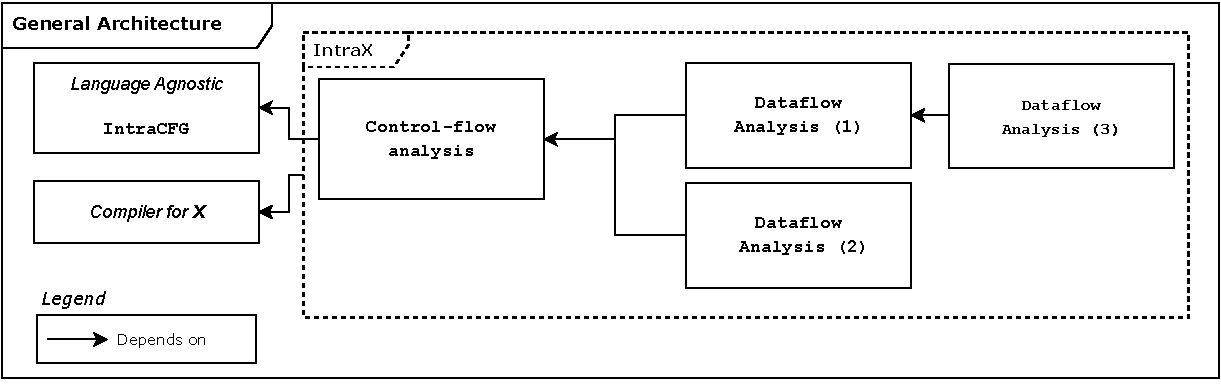
\includegraphics[scale=0.7]{kappa/img/architecture.pdf}
	\caption{\label{fig:intraCFG} Overall architecture of \textsc{IntraCFG} and its ecosystem.}
\end{figure}

The framework consists of several key components, including interfaces
(e.g., CFGRoot, CFGSupport, and CFGNode), attribute equations that define the
default behavior, and user APIs. The interfaces provide the structure for the
CFG and the attribute equations define the default behavior for the CFG
construction. Language specific AST nodes implement the different interfaces 
according to the level of precision desired for the CFG.
The APIs expose the CFG to the client analysis, and they are used to query the CFG
for information, such as the entry and exit nodes, or to traverse the CFG.
The language-independent nature of \textsc{IntraCFG} allows for easy integration 
with various programming languages and enables the construction of precise CFGs 
for those languages. The use of attribute equations and interfaces also allows 
for a high degree of flexibility in the CFG construction process, 
enabling the customization of the CFG to fit the specific needs of the 
analysis being performed.

Additionally, language-specific dataflow analysis, such as NullPointerException or
IndexOutOfBound detection, can be built on top of the framework.
\subsection{\textsc{IntraCFG} for Java}
\begin{figure}[H]
	\centering
	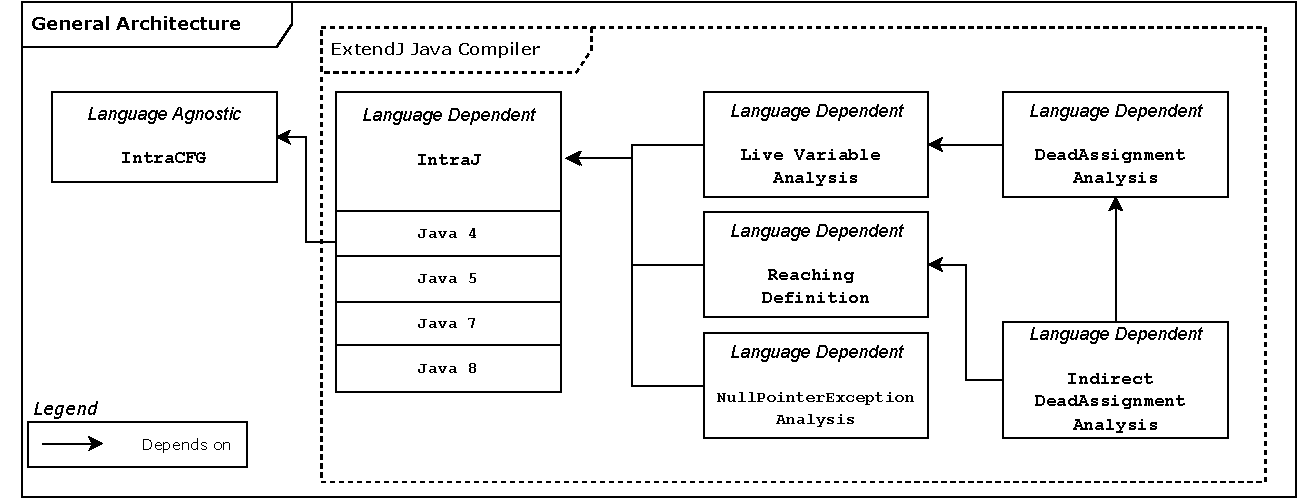
\includegraphics[scale=0.5]{kappa/img/architecturejava.pdf}
	\caption{\label{fig:intraJ} Overall architecture of \textsc{IntraCFG} instansiated for the Java language.}
\end{figure}

\subsection{\textsc{IntraCFG} for TEAL}
\begin{figure}[H]
	\centering
	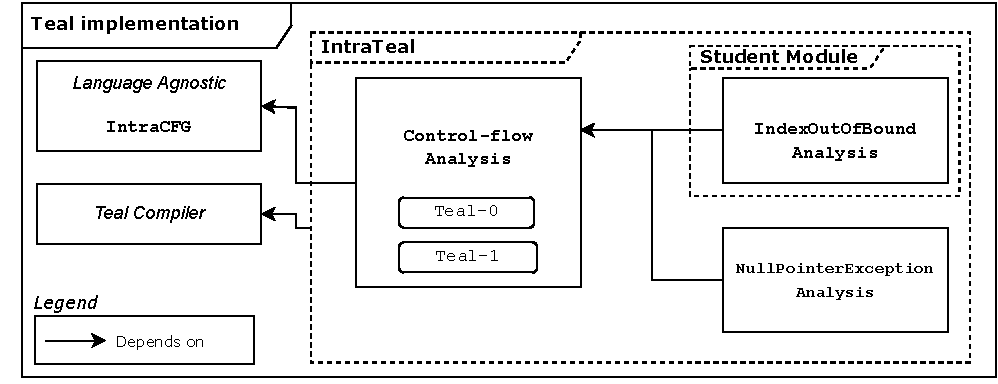
\includegraphics[scale=0.65]{kappa/img/architectureteal.pdf}
	\caption{\label{fig:IntraTeal} Overall architecture of \textsc{IntraCFG} instansiated for the Teal language.}
\end{figure}
\subsection{IDE Integration}
\subsubsection{LSP support via MagpieBridge: showing results and fixes}

\subsubsection{Visualisation and debugging via Codeprober}



\section{JFeature: A Java Feature Extractor}






\label{sec:contribution}
In this Thesis, we present two major contributions to the field of programming 
language analysis and software engineering. 
The first significant contribution of this thesis is the formalisation of \textsc{IntraCFG},
a language-agnostic RAG-based framework for constructing control-flow graphs (CFGs) 
on top of the abstract syntax tree (AST). \textsc{IntraCFG}, is a highly flexible
framework that enables the construction of light-weight and precise the control-flow graphs
of a program. To exemplify the applicability of \textsc{IntraCFG}, we instantiate it for the TEAL language.

The second contribution is a Java feature extractor called \textsc{JFeature}.
This tool is designed to assist researchers in selecting the appropriate corpora
for their experiments by extracting relevant features from Java programs. 
\textsc{JFeature} is able to extract a wide range of features, 
including syntactic, e.g., use of keywords, and semantic features, e.g.,
the number of method calls.


\subsection{\textsc{IntraCFG}: A Precise Framework for Source-level Control-flow Analysis}

\subsubsection*{Design and Implementation}
\textsc{IntraCFG} is written within the \textsc{JastAdd} ecosystem.

The framework provides three interfaces, namely \code{CFGRoot}, \code{CFGNode}, and \code{CFGSupport},
to be implemented by AST nodes. Each interface provides a set of attribute that are used to construct
the CFGs.

The \code{CFGRoot} interface is the starting point of the CFG construction process.
It is implemented by AST nodes that identify the subtree containing the entire method 
or function. This interface is responsible for defining the entry and exit nodes of the CFG and 
forwards a reference of the entry node to every \code{CFGNode}.


The \code{CFGSupport} interface is implemented by nodes that are not part of the CFG,
but define its shape. These nodes are used to provide additional information 
about the structure of the CFG, such as the presence of loops or branches. 
They are designed to be used as auxiliary nodes to support the CFG construction 
process, and they do not participate directly in the control-flow.